\documentclass{birkjour}

\usepackage{tikz}
\usepackage{graphicx}
\usepackage{hyperref}

\newtheorem{thm}{Theorem}[section]
\newtheorem{cor}[thm]{Corollary}
\newtheorem{lem}[thm]{Lemma}
\newtheorem{prop}[thm]{Proposition}
\theoremstyle{definition}
\newtheorem{defn}[thm]{Definition}
\theoremstyle{remark}
\newtheorem{rem}[thm]{Remark}
\newtheorem*{ex}{Example}
\numberwithin{equation}{section}

\newcommand{\R}{\mathbb{R}}
\newcommand{\B}{\mathbb{B}}
\newcommand{\G}{\mathbb{G}}
\newcommand{\V}{\mathbb{V}}
\newcommand{\gd}{\dot{g}}
\newcommand{\gh}{\hat{g}}
\newcommand{\Gd}{\dot{G}}
\newcommand{\Gh}{\hat{G}}
\newcommand{\nvai}{\infty}
\newcommand{\nvao}{o}
\newcommand{\grade}{\mbox{grade}}

\begin{document}

%-------------------------------------------------------------------------
% editorial commands: to be inserted by the editorial office
%
%\firstpage{1} \volume{228} \Copyrightyear{2004} \DOI{003-0001}
%
%
%\seriesextra{Just an add-on}
%\seriesextraline{This is the Concrete Title of this Book\br H.E. R and S.T.C. W, Eds.}
%
% for journals:
%
%\firstpage{1}
%\issuenumber{1}
%\Volumeandyear{1 (2004)}
%\Copyrightyear{2004}
%\DOI{003-xxxx-y}
%\Signet
%\commby{inhouse}
%\submitted{March 14, 2003}
%\received{March 16, 2000}
%\revised{June 1, 2000}
%\accepted{July 22, 2000}
%
%
%
%---------------------------------------------------------------------------

\title{The Intersection Of Rays With\\Algebraic Surfaces}

\author{Spencer T. Parkin}
\address{102 W. 500 S., Salt Lake City, UT  84101}
\email{spencerparkin@outlook.com}

\subjclass{Primary 14J70; Secondary 14J29}

%\date{October 22, 2013}

%\dedicatory{To my dear wife Melinda.}

\begin{abstract}
Although a well known\footnote{See the generalized Taylor series in \cite{Weisstein13}.}
result in the traditional language of multi-variable calculus,
in this paper it is shown, using the language of geometric algebra, that for any
real-valued polynomial defined over $n$-dimensional euclidean space, that
the image of any line through the domain of such a function
is determined entirely by all orders of directional derivatives of this function at
any one point along the line and in the direction of the line.

This result has an
application in the problem of casting rays through algebraic surfaces as it
shows that such a problem, in all cases, reduces to the problem of finding
the roots of a real-valued polynomial in one real variable, and having an explicit formulation
in terms of the surface and ray in question.

A generalization of the gradient is found in geometric algebra that is
similar to differential forms.
\end{abstract}

\maketitle

\section{Introduction}

This paper uses the framework laid out in \cite{Parkin13} for the representation of
algebraic surfaces, and so assumes sufficient knowledge of that work.
What may be worth revisiting here at the start, however, is an additional
conception of the notation used in that paper; specifically to do with the
heavy use of subscripts.  This paper is no exception to such use of subscripts,
and so the reader must be up to speed on the notation if there is
to be any hope of success in communicating the ideas to follow.

Unless otherwise specified, a subscript denotes membership in a
specific sub-algebra.  These sub-algebras of our ``mother'' algebra $\G$ are
enumerated by the
integers in $[1,m]$, and denoted by $\G_i$.  The absence of a subscript
can denote membership in an algebra or space outside of $\G$,
usually $\R^n$, which is thought of as an $n$-dimensional euclidean vector
space.

This, however, does not have to be the case, and we can work exclusively
in $\R_1^n$, a sub-space of the vector space $\V_1$ generating $\G_1$.
The omission of a subscript, (or, as usual, the presence of the subscript 1),
can denote membership in $\G_1$, while the
presence of a subscript can be thought of as the application of an
outermorphism\footnote{An explicit formula for this
outermorphism was given in the appendix of \cite{Parkin13}.}
 that takes us from $\G_1$ to the corresponding element
in $\G_i$, $i$ being the subscript in question.  This being the
conception of our use of subscripts, they may begin to play a role
in our performance of certain algebraic manipulations, such as
\begin{align*}
(a+b)_i &= a_i + b_i, \\
(a\wedge b)_i &= a_i\wedge b_i, \\
a\cdot b &= a_i\cdot b_i, \\
a_i\cdot a_j &= 0, \\
a_i\wedge a_j &\neq 0, \\
(a_i)_i &= -a,
\end{align*}
with $a,b\in\V_1$ and $i\neq j$.  Except for the last, these are all important properties
of the algebra that make the representation scheme work.
In the remainder of this paper, you may think of $\R^n$ as $\R_1^n$ if you would like.
In any case, the reader must understand the application of subscripts to otherwise
unsubscripted variables and expressions.  This is covered in detail in \cite{Parkin13}.

\section{An Approach To The Problem}

Letting $f:\R^n\to\R$ be any polynomial equation in $n$ variables and up to degree $m$, it
was shown in \cite{Parkin13} that the function $\bigwedge_{i=1}^m p_i(x)$ may be factored out
of this polynomial in terms of the inner product as
\begin{equation}\label{equ_polynomial_func}
f(x) = \bigwedge_{i=1}^m p_i(x)\cdot B,
\end{equation}
where $B$ is an $m$-vector of our geometric algebra with $\nvai_i\cdot B=0$ for all
integers $i\in[1,m]$, and where the function
$p_i:\R^n\to\V_i$ is given by
\begin{equation}\label{equ_point_func}
p_i(x) = \nvao_i + x_i + \frac{1}{2}x_i^2\nvai_i,
\end{equation}
having its origins in the paper \cite{Hestenes01}.
Given a point $x\in\R^n$ and a direction vector $v\in\R^n$,
we wish to find the set of all scalars $\lambda\in\R$ such that $f(x+\lambda v)=0$.
Utilizing equation \eqref{equ_polynomial_func} for this purpose, we easily find that
\begin{equation}\label{equ_ray_polynomial_unexpanded}
f(x+\lambda v) = \bigwedge_{i=1}^m(p_i(x)+\lambda v_i)\cdot B,
\end{equation}
because we can ignore the $\frac{1}{2}x_i^2\nvai_i$ term in equation \eqref{equ_point_func}
on account that $\nvai_i\cdot B=0$.
Looking at equation \eqref{equ_ray_polynomial_unexpanded},
it is immediately clear that its expansion is that of a polynomial in $\lambda$ of up to degree $m$.
What we're going to show in this paper is that an explicit formula for this polynomial can
be found in terms of all orders of directional derivatives of $f$ at $x$ and in the
direction of $v$.

\section{The Result}

We begin by rewriting equation \eqref{equ_ray_polynomial_unexpanded} as
\begin{equation}\label{equ_ray_polynomial_expanded_but_unknown}
f(x+\lambda v) = \sum_{i=0}^m T_i(x),
\end{equation}
where $T_i(x)$ will denote the $i^{th}$ term collecting all multiples of
$\lambda^i$ in the series expansion of
\eqref{equ_ray_polynomial_unexpanded}.  Carefully formulating this term, we get
\begin{equation*}
T_i(x) = \lambda^i \sum_{j=1}^{\binom{m}{i}} W_{j,i}(x)\cdot B,
\end{equation*}
where $W_{j,i}$ is the $j^{th}$ way to write an outer product involving
$i$ vectors taken from $\{v_k\}_{k=1}^m$ and $m-i$ vectors taken from
$\{p_k(x)\}_{k=1}^m$ in an order having ascending sub-scripts.  The following
example helps clarify this in the case $m=3$.
\begin{align*}
W_{1,0} &= p_1\wedge p_2\wedge p_3 \\
W_{1,1} &= p_1\wedge p_2\wedge v_3 \\
W_{2,1} &= p_1\wedge v_2\wedge p_3 \\
W_{3,1} &= v_1\wedge p_2\wedge p_3 \\
W_{1,2} &= p_1\wedge v_2\wedge v_3 \\
W_{2,2} &= v_1\wedge p_2\wedge v_3 \\
W_{3,2} &= v_1\wedge v_2\wedge p_3 \\
W_{1,3} &= v_1\wedge v_2\wedge v_3
\end{align*}
Having now come to terms, (no pun intended), with the general expansion of
equation \eqref{equ_ray_polynomial_unexpanded}, we proceed now to
fearlessly take the directional derivative of $T_i$ at $x$ and in the direction of $v$.
Doing so, we get
\begin{align*}
\nabla_v T_i(x) &= \lambda^i\sum_{j=1}^{\binom{m}{i}}\lim_{\delta\to 0}
\frac{W_{j,i}(x+\delta v)-W_{j,i}(x)}{\delta}\cdot B,
\end{align*}
knowing that each individual limit will exist.  What we must realize now is that
the term $W_{j,i}(x)$ will get canceled in the expansion
of $W_{j,i}(x+\delta v)$, leaving only terms that are multiples of positive powers of $\delta$.
Furthermore, it is only those remaining terms that are multiples of $\delta$ itself
that will survive the limit process.  We are therefore left to deduce these terms in an
evaluation of the limit.  What we find is that all such terms are of the form
$\delta W_{j,i+1}(x)$, but we need to determine just how many of them there are.
Realizing that $\binom{m}{i}$ old terms will each contribute $m-i$ new terms of
this form, of which there should be $\binom{m}{i+1}$, but that no type of term
will be produced any more or less than any other, we see that
\begin{equation*}
\frac{(m-i)\binom{m}{i}}{\binom{m}{i+1}}=i+1
\end{equation*}
is the number of such terms of the form $\delta W_{j,i+1}(x)$, and we may write
\begin{align}
\nabla_v T_i(x) &= \lambda^i\sum_{j=1}^{\binom{m}{i+1}}\lim_{\delta\to 0}
\frac{(i+1)\delta W_{j,i+1}(x)}{\delta}\cdot B\nonumber \\
 &= \lambda^i(i+1)\sum_{j=1}^{\binom{m}{i+1}} W_{j,i+1}(x)\cdot B\nonumber \\
 &= \frac{i+1}{\lambda}T_{i+1}(x).\label{equ_recurrence_relation}
\end{align}
Returning to equation \eqref{equ_ray_polynomial_expanded_but_unknown},
and realizing that $T_0(x)=f(x)$, we can now finally deduce the expansion of
\eqref{equ_ray_polynomial_unexpanded} using the recurrence relation
of equation \eqref{equ_recurrence_relation} as
\begin{equation}\label{equ_result}
f(x+\lambda v) = \sum_{i=0}^m\frac{\lambda^i}{i!}\nabla_v^i f(x),
\end{equation}
where $\nabla_v^i f(x)$ is the $i^{th}$ order directional derivative of $f$ at $x$
in the direction of $v$ with $\nabla_v^0 f(x)=f(x)$.

Clearly this is a Taylor series, and so a much simpler
derivation could have probably been found, perhaps using the
concept of integration along the ray.  In any case, we have been
able to show the promised result.

\section{Making Use Of The Result}

\begin{figure}
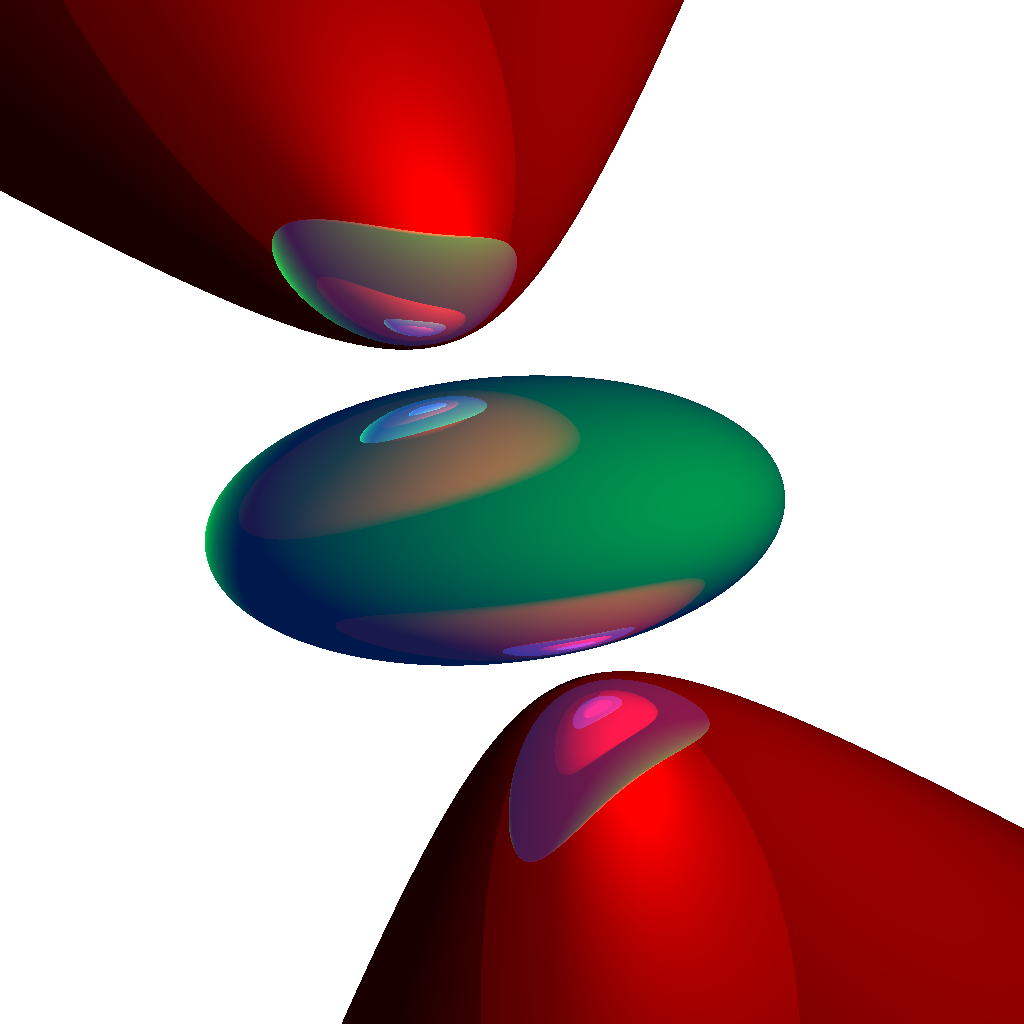
\includegraphics[scale=0.3]{Quadrics}
\caption{An ellipsoid and a hyperboloid of two sheets ray-traced by finding the zeros
of the quadratic equation found through the use of equation \eqref{equ_result_decoupled}.
The ray-tracing software used here can be found at \url{https://github.com/spencerparkin/ImageGenerator}.}
\label{fig_ray_traced_image}
\end{figure}

In its present form, equation \eqref{equ_result} lacks ease of use, because knowledge of the
vector $v$ is needed to calculate all positive orders of the directional derivative.  To solve this problem,
we need to decouple the knowledge of this vector from the limit processes by generalizing the
idea of the gradient to higher orders.

We begin with the gradient of $f$, usually written $\nabla f$, but this is ambiguous in our algebra,
because we need to specify the sub-algebra over which $\nabla f$ will be taken.  We will
do this with an integer subscript as $\nabla_i f$, not to be confused with the directional
derivative, which uses a vector subscript.  The gradient can now be defined similarly to
it's definition in \cite{Macdonald12} as
\begin{equation}\label{equ_gradient_func_operator}
\nabla_i = \sum_{j=1}^n e_{i,j}\nabla_{e_j},
\end{equation}
where $\{e_{i,j}\}_{j=1}^n$ is an orthonormal basis for $\R^n_i$, and
we, for all integers $i\in[1,n]$, let $e_i=e_{1,i}$ for convenience.
Having done this, we have, for any integer $i\in[1,m]$,
\begin{equation*}
\nabla_v = v_i\cdot\nabla_i,
\end{equation*}
which is a well-known result.  Generalizing this, we find that
\begin{equation}\label{equ_generalize_gradient_func_operator}
\nabla_v^i = -(-1)^i\bigwedge_{j=1}^i v_j\cdot\bigwedge_{j=1}^i\nabla_j,
\end{equation}
where the function operator $\bigwedge_{j=1}^i\nabla_j$ is defined as
\begin{equation}\label{equ_expand_func_operator}
\bigwedge_{j=1}^i\nabla_j =
\sum_{j_1=1}^n\dots\sum_{j_i=1}^n\left(\bigwedge_{k=1}^i
e_{k,j_k}\right)\prod_{k=0}^{i-1}\nabla_{e_{j_{i-k}}}.
\end{equation}
Here, the function operator on the right-hand side of equation \eqref{equ_expand_func_operator}
is an $i^{th}$ order partial derivative.
If not for the reverse order of partial derivatives, equation \eqref{equ_expand_func_operator}
would have been omitted on
the basis that equations \eqref{equ_gradient_func_operator} and
\eqref{equ_generalize_gradient_func_operator}, together, sufficiently
define the operator $\bigwedge_{j=1}^k\nabla_j$.  Those two equations
probably are sufficient, however, if we realize how the composition of operators, as a product,
must be taken.  In any case, \eqref{equ_expand_func_operator} is given for clarity and comparison
against equation \eqref{equ_gradient_func_operator} as a generalization of it.

Notice that this generalization of the gradient appears in keeping with the reoccurring theme
of grade raising or lowering operations found in geometric algebra.  The traditional gradient,
as we knew it, raised the grade of scalar-valued functions to that of vector-valued functions.
The more general gradient we have in \eqref{equ_generalize_gradient_func_operator} now raises a scalar-valued function to that
of an $i$-blade-valued function.
For an $i$-blade-valued function, the function $\nabla_j\wedge f$ has the potential to be
an $(i+1)$-blade-valued function, while the function $\nabla_j\cdot f$ has that of
an $(i-1)$-blade-valued function.

Definition \eqref{equ_expand_func_operator} is comparable to the
definitions given in \cite{Hestenes93,Macdonald12} for differential forms.
Definition \eqref{equ_generalize_gradient_func_operator} strives to be coordinate free.
The main difference between \eqref{equ_expand_func_operator} and differential forms
is that such forms, in the context of our algebra $\G$, are restricted to a single sub-algebra.

Returning from a brief digression, the decoupling of equation \eqref{equ_result} can now be written as
\begin{equation}\label{equ_result_decoupled}
f(x+\lambda v) = -\sum_{i=0}^m\frac{(-\lambda)^i}{i!}\bigwedge_{j=1}^i v_j\cdot\left(\bigwedge_{j=1}^i\nabla_j\right)f(x),
\end{equation}
where the outer product $\bigwedge_{j=1}^i v_j$ is one in the case $i=0$, and where the function
operator $\bigwedge_{j=1}^i\nabla j$ is the identity operator in the same case.

If all orders of the gradient of $f$ are available to us, equation \eqref{equ_result_decoupled} becomes
a convenient way to calculate the coefficients of the polynomial whose zeros give us the parameters of
the intersection points of our ray with a given algebraic surface.

Looking back again at equation \eqref{equ_ray_polynomial_unexpanded}, this is certainly a usable form
if a symbolic calculator is available.  Use of symbolic calculation was made in \cite{Hanrahan83}.  If no such
thing is available, then \eqref{equ_result_decoupled} allows us to come up with the polynomial
through literal evaluation; provided, again, that we have all gradients available to us.
For algebraic surfaces of degrees greater than or equal to five,\footnote{There is no closed form solution
to a general polynomial of degree greater than or equal to five in terms of elementary functions.  See \cite{Gallian12}.} we may
lose the need to come up
with the polynomial expansion of $f(x+\lambda v)$ altogether in favor of root-finding methods
that need know nothing more about $f(x+\lambda v)$ other than that it is continuous on
a compact interval.\footnote{In such a
case, the intermediate value theorem applies.  Recall that the composition of two continuous functions
is continuous.}

In any case, \eqref{equ_result_decoupled} appears to be, if nothing more, an
interesting result about scalar fields that may find applications in other areas.
Figure~\ref{fig_ray_traced_image} shows an application to ray-tracing.

Notice that \eqref{equ_result} stands on its own, independent of the framework
of \cite{Parkin13}, or even geometric algebra itself.  There does not appear,
however, to be an easy way, if at all, to decouple \eqref{equ_result} using
differential forms as we have in equation \eqref{equ_result_decoupled},
which depends upon the said framework in which we have the generalized gradient
of equation \eqref{equ_generalize_gradient_func_operator}.

\bibliographystyle{amsplain}
\bibliography{Parkin_TheIntersectionOfRaysWithAlgebraicSurfaces}

\end{document}